\documentclass[buriama8_dp.tex]{subfiles}
\begin{document}

\chapter{Robotic hardware and framework}

\section{ROS}
\label{sec:ros}

The arm (and the whole TRADR robot) run under the \emph{Robot Operating System} – ROS \cite{ros_paper}. This framework allows us to build robot software in a very modular fashion by providing us with standardized units (\uvz{nodes}) and M-to-N communication links (\uvz{topics}). Each hardware component of the robot (e.g. a LIDAR or a motor driver) has its own driver node, and so does each functional software part (mapping, adaptive traversability etc.). In ROS, we can put these ready-made parts together easily and run them in a distributed fashion, as each node can run on a different computer and the system will automatically relay the information between the hosts. The modularity also guides us to design small and manageable pieces of software that integrate well with the rest of the environment and provide the new functionality we want.

The ROS framework is only a common interface specification, with the actual implementation of a node completely independent on other nodes. Each node can be implemented in a different programming language, as long as they conform with the communication standards.

Nodes run in event loops, referred to as \emph{spinning}. In each loop iteration, an event is taken from the incoming event queue and the appropriate callback is issued.

\subsection{ROS primitives}
\label{subsec:ros_prims}

Basic unit of information in ROS are \emph{messages}. A message is a tuple with named values of different types, possibly other messages. A Pose message, representing position and orientation of an object in space, contains a Position message (which in turn contains \m x, \m y, and \m z coordinates as floating point numbers) holding the information about the position of the object, and a Quaternion representing its orientation.

The basic communication links are \emph{topics}. Nodes write messages to topics, and other nodes can subscribe to the topics and consume messages from them. For example a sensor driver node publishes the sensor measurements for the rest of the system to use.

The second communication primitive provided by ROS core are \emph{services}. Services implement request-response behavior, when a client calls the service provided by a node and receives a response for its request. For example, a laser range meter driver could be implemented as a service, accepting requests for measurement and returning the outcome.

\subsection{Actions}
\label{subsec:ros_actions}

On top of these primitives, another interface type is implemented, the \emph{actions}. Actions are not a part of core ROS as topics and services, but have become a standard part of ROS interfaces.

Actions consist of a set of topics and and are similar to services. A client sends a request to the action server. The action server then sends feedback back to the client as it performs the requested action. When the server is done, the client is notified by a goal message.

A good example for an action server is one for driving the robot to a defined pose. The action server receives a Pose message and sets off. As the robot is under way, the server sends periodic updates on the current pose back to the client. When the final pose is reached, the server notifies the client that the work is done together with optional complimentary data, like the length of the path taken.


\section{Kinova JACO}
\label{sec:jaco}
We will be working with the Kinova JACO robotic arm. It is a 6 degrees of freedom lightweight robotic arm, designed by Kinova Robotics for use in assistive and collaborative applications. Originally designed to be used in assistive robotics, mounted on mobile structures as wheelchairs, JACO's lightness makes it ideal for uses on mobile robots \cite{kinova}.

\begin{figure}[ht]
  \centering
  \hspace{1cm}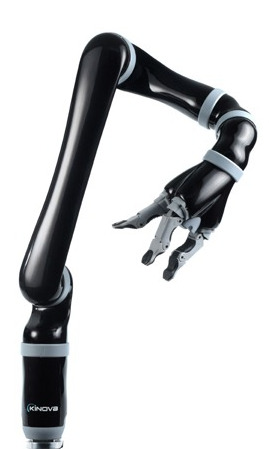
\includegraphics[width=4cm]{jaco.jpg}
  \caption{The Kinova JACO 6DOF robotic arm with the 3-finger gripper. Photo taken from \cite{kinova}}
  \label{fig:jaco}
\end{figure}



\subsection{Serial manipulator}
\label{subsec:arm_theory}

The JACO arm is a serial manipulator, meaning that it is a chain of links interleaved with joints. A movement in a joint affects all the following joints and links in the chain. The base of the chain is often a fixed base, while the tip of the chain is reffered to as the \emph{end effector}. The positional behavior of the arm is referred to as arm kinematics.

The compound joint and link transformations (rotations and translations, respectively) links the joint configuration to the end effector pose (as user in ROS terminology, representing position \(\vec p\) and orientation \(\vec r\)). Computation of the end effector pose from joint angles \(\vec q = (q_1 \ldots q_n)\), a column vector where \m n is the number of joints, is referred to as \emph{Forward Kinematics -- FK} computation. From now on, we consider a 6DOF manipulator like JACO.

The inverse problem is finding joint values that reach the given end efffector pose, and is called \emph{Inverse Kinematics - IK}. As many inverse problems, it is considerably harder to solve than the forward problem \cite[sec. 2.12]{manipulators}; it is often solved numerically.

When not positions, but velocity of the end effector and joints is studied, it is in the field of differential kinematics. The relation between the joint angular velocities \(\dot{\vec q}\) and end effector pose velocity (usually called \emph{twist})
\[\vec v = \colvec{\dot{\vec p}}{\vec \omega},\]
where \(\dot{\vec p}\) represents linear velocity and \(\vec \omega\) anglular velocity, is described by the Jacobian matrix \(\mat J(\vec q) \in \R^{6 \times 6}\) of the manipulator:
\[
  \vec v = \mat J(\vec q)\dot{\vec q}
\]

The inverse problem is again considerably harder, as it involves inverting the Jacobian (if it is regular). As inversions in possibly near singular matrices are numerically unstable, pseudoinverse that deal with singularities is often used.

\subsection{Arm kinematics}
\label{subsec:arm_kinematics}

The arm has slightly unusual geometry in its wrist. The wrist is not spherical (the axes of its joints do not intersect in one point), which means that positioning the arm in a given pose cannot be separated into position and orientation problems. Usage of some inverse kinematics solvers that count on this is thus impossible.

Instead, the wrist consists of three revolute joints that have angular offsets of \(60\degr\) (see Figure~\ref{fig:jaco_schema}). This limits the workspace where the arm has full 6DOF capabilities, as the rotation of the wrist is limited; however, the arm exhibits this limitations only in extreme poses.

\begin{figure}[ht]
  \centering
  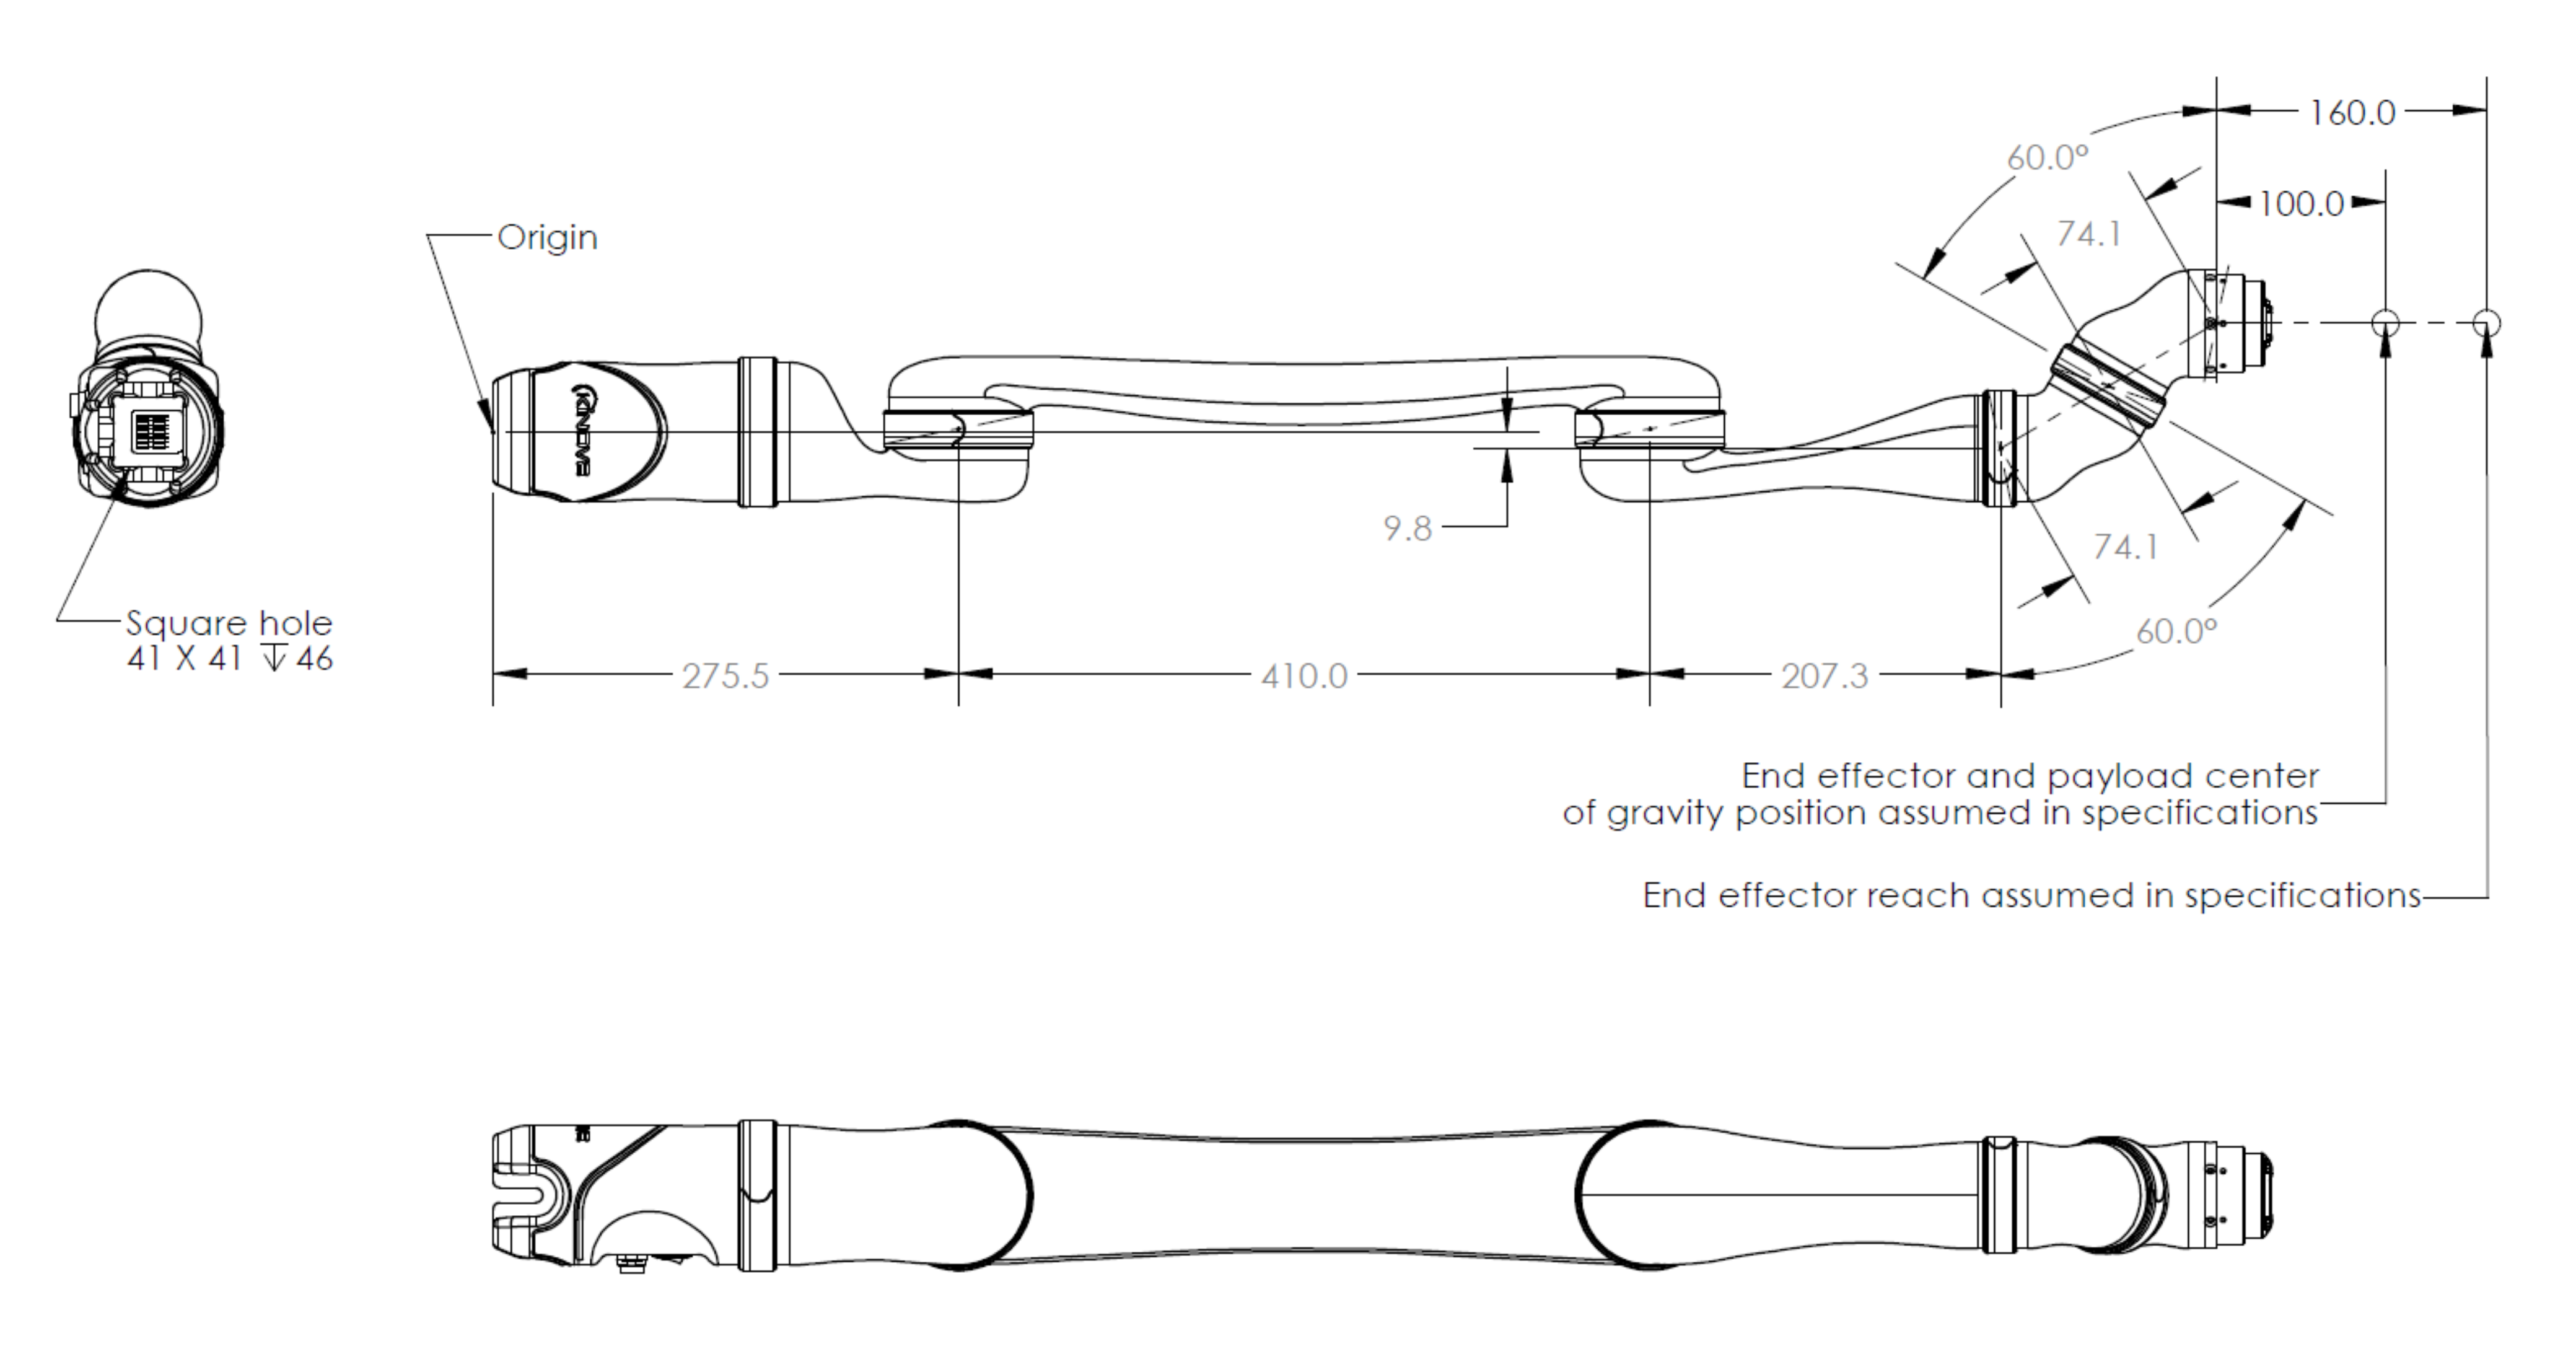
\includegraphics[width=\textwidth]{jaco_spec_drawing.png}
  \caption[JACO blueprint]{JACO arm technical specification. Note the wrist (last three joints) construction that limits the end effector orientation. Taken from \cite{jaco_spec}}
  \label{fig:jaco_schema}
\end{figure}

The arm manufacturer states the reach of the arm is 90\,cm. The arm (including the gripper) can actually reach beyond 100\,cm, but only with limited rotation. In the 90\,cm work range, a wide range of hand orientations is still possible. On the other side, the arm cannot reach all orientations if the end effector is close to the base. We observed that to reach closer than 40\,cm and point the gripper away from the base, the arm needs to be in extreme poses, which are better avoided as they bring the arm close to self-collision.

\subsection{Kinova ROS driver}
\label{subsec:kinova_ros}

The manufacturer provides an open-source ROS library to operate the arm \cite{kinova_ros}. The driver runs a node that communicates with the arm via a USB interface and relays incoming commands from other components. The driver is an evolution of a former JACO ROS driver that supported only the JACO arm. Recently, Kinova replaced the JACO-specific driver with the new one, which supports also other Kinova arms.

The driver provides interfaces to moving the arm to joint space and Cartesian space targets, controlling fingers of the gripper and directly driving Cartesian velocity of the end effector and angular velocities of each joint \cite{kinova_ros_api}. It also provides two utility services for homing the arm and for stopping all movement immediately.

\subsection{Cartesian and joint space targets}
\label{subsec:api_cart_action}

Driving the arm to joint space and Cartesian space targets is possible via the respective action servers. The action servers accept Pose, resp. JointAngles message describing the desired target state. They report the current position back as the movement proceeds, and in the end return the actual pose the arm ended in. For the Cartesian pose target, no IK computation is performed by the driver itself, the target pose is only fed into the arm and the internal control algorithms take care of the rest. The movement also does not take any obstacle avoidance or collision prevention into account, except self-collisions that are checked. This renders the features practically unusable if we know there are obstacles in the environment.

\subsection{Cartesian and joint space velocity}
\label{subsec:api_cart_vel}

Controlling the arm movement via directly specifying velocities is implemented quite differently. To set Cartesian or joint angular velocities, the client publishes a message to a specified topic. The driver then forwards the message to the arm, where it is consumed from a queue by the arm's control algorithm. The control algorithm runs at 100\,Hz, and sets the velocity for the next iteration from the queue. Thus, once the client stops publishing to the topic, the movement stops immediately. The control is arguably implemented this way to minimize latency of stopping any movement. It also means, that to set the velocity for a longer time, the client needs to publish to the velocity control topic periodically at 100\,Hz. With lower frequency, the movement will be jagged, as some control loop iterations will set zero velocity. If the frequency were higher, the input queue of the arm would overflow, causing the arm to stall.

\subsection{Utility services}
\label{subsec:api_util}

Homing the arm is possible by calling a home service in the ROS driver. The home pose can be adjusted in the arm firmware by Kinova's arm controlling software.

The stop service stops all movements of the arm immediately. To resume operation, the arm must be started again by calling a start service. When restarted, all commands that came after stopping are dropped and need to be re-issued if they are to be carried out.

%%%
\section{MoveIt!}
\label{sec:moveit}

The ROS framework was primarily designed to operate whole mobile robots; it is not so well suited to control robotic manipulators. To help in this area, the MoveIt! package \cite{moveit_docs} was designed to facilitate this task. It encompasses the full stack necessary to operate a robotic arm, from managing the state of the scene, through manipulation, motion planning, collision-checking, IK solving to outputting commands that can be used directly to control a manipulator.

\subsection{MoveIt! architecture}
\label{subsec:mvt_arch}

MoveIt runs a large monolithic node called move group. The move group is responsible for all the operations of the arm. It consumes the state of the arm (joint angles) from the driver, as well as commands from the user issued via client libraries. The architecture is illustrated in Figure~\ref{fig:moveit_arch}.

\begin{figure}[ht]
  \centering
  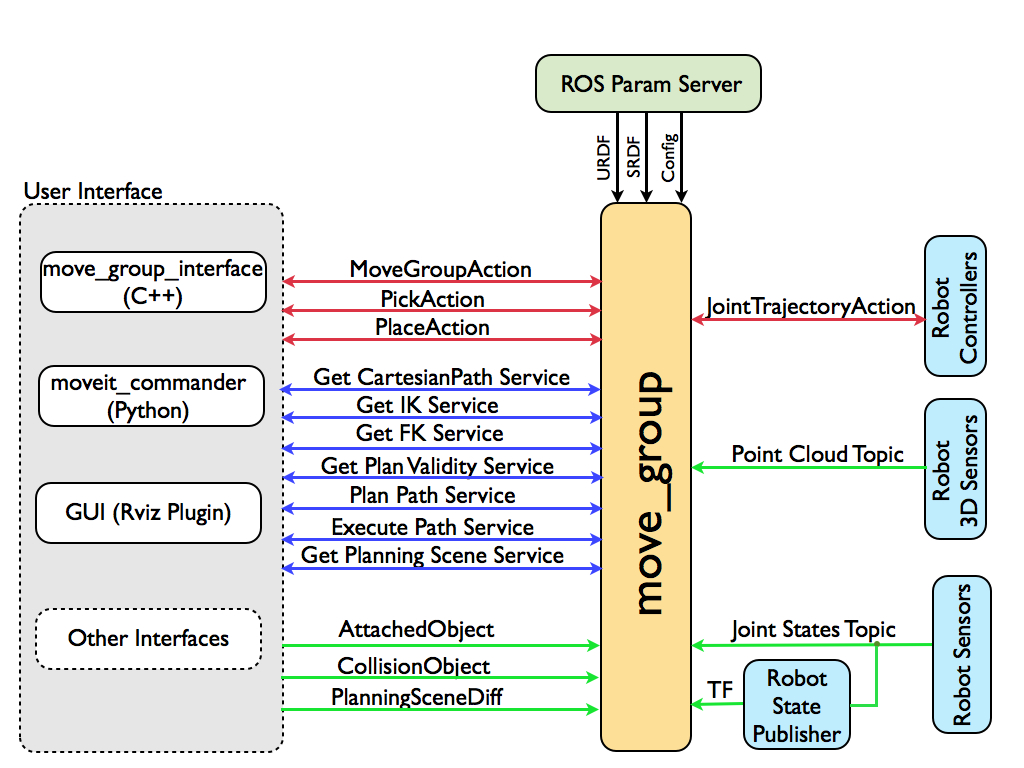
\includegraphics[width=.9\textwidth]{moveit_arch}
  \caption[MoveIt! architecture]{Illustration of MoveIt! architecture. Taken from \cite{moveit_docs}}
  \label{fig:moveit_arch}
\end{figure}

The central node represents the move\_group, which listens to input from the robot hardware in the lower right, as point cloud sensors and introceptive sensors. It outputs commands to the manipulator to the controller with \code{JointTrajectoryAction} interface and is controlled by the inputs on the left. MoveIt has a plugin-oriented extensible architecture, where all services like IK solving and motion planning are defined as plugins, interchangable with other implementations.

\subsection{User interface}
\label{subsec:moveit_ui}

The user interface, or client libraries, for MoveIt are prepared in C++ and python. The libraries contain objects and utility functions to use the functionality of the move group and communicate with the move group via its ROS topic and service interface. All the interfaces and functionalities are very poorly documented, and the best available resources are the automatically generated code documentation and the source code itself. The client libraries can be used directly to access the motion planning capabilities to reach some higher-level goals.


\subsection{Robot interface}
\label{subsec:moveit_ri}

MoveIt interfaces with the robot hardware by an action server implementing the \code{JointTrajectoryAction}. The server then drives the arm hardware. The \code{JointTrajectoryAction} is specified as a trajectory in space of joint angles and velocities, prepared by the motion planner with respect to both the arm kinematics (preventing collisions) and the arm dynamics (taking limits on joint velocities into account). The trajectory waypoints specify both the desired joint angles, as well as joint velocities necessary to reach the next waypoint. Each waypoint also specifies a point in time in which the arm should have reached it.

In case of the Kinova ROS driver, no such server is provided by the manufacturer. A pull request (code contributed by a developer) on GitHub containing this functionality exists, but is not a part of the release yet. We used an implementation of this server by Matěj Balga \cite{matej} , which we updated to work with the newest drivers from Kinova. The server is rather simplistic. It follows the joint velocities defined in the waypoints, forwarding them to the arm driver for as long as the waypoint specifies.

At the trajectory end, the current arm joint pose is compared to the desired final pose. If they are different, a simple P regulator is used to move the arm joints to within tolerance of the final positions. This behavior is very apparent after following a more complex trajectory, which includes many direction changes. It could prove dangerous for the arm when maneuvering in proximity of obstacles, as the arm strays off the collision-free trajectory. The final movement is also very fast, and could damage the arm if anything were to happen. We assume this happens because the driver forwards the velocities to the arm directly, without taking accelerations into account. The arm firmware has acceleration limits built in, and when the limit is applied and the set velocity is truncated, the actual arm position diverges from the position expected by the driver.

The driver could possibly be improved by interpolating the velocities on a spline rather than linearly, smoothing out the velocity changes and thus not letting the arm firmware to interfere with the control.

\subsection{Inverse Kinematics solver -- TRAC-IK}
\label{subsec:tracik}

During our initial experiments with the arm, we encountered puzzling behaviors of the motion planners. The arm would sometimes move along a seemingly random, unnecessarily long path. At closer investigation, we concluded that the planning was actually optimal, but what was wrong was the Inverse Kinematic (\emph{IK}) solution for the target pose. Such plan is illustrated in Figure~\ref{fig:wrong_planning}.

Because of the slightly non-standard arm kinematics (see section \ref{subsec:arm_kinematics}), the default IK solver used by MoveIt (the KDL numerical solver) would sometimes produce a solution that indeed reaches the desired end effector pose, but that is very far in joint space from the current joint state (e.g. the first joint is rotated), even when a very small end effector motion is required.

\begin{figure}[htp]
  \centering
  \begin{subfigure}[t]{0.49\textwidth}
    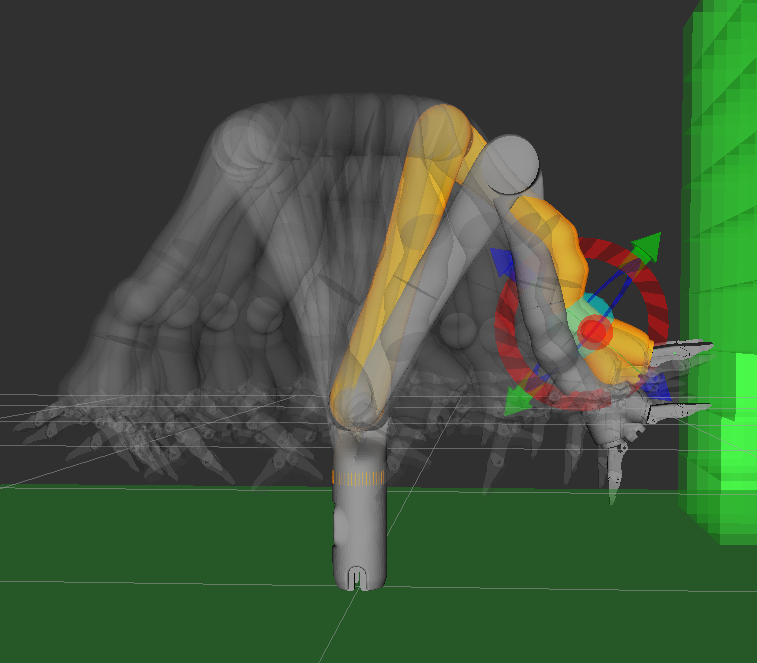
\includegraphics[width=\textwidth]{wrong_plan.png}
    \caption{}
    \label{fig:wron_plan}
  \end{subfigure}
  \begin{subfigure}[t]{0.49\textwidth}
    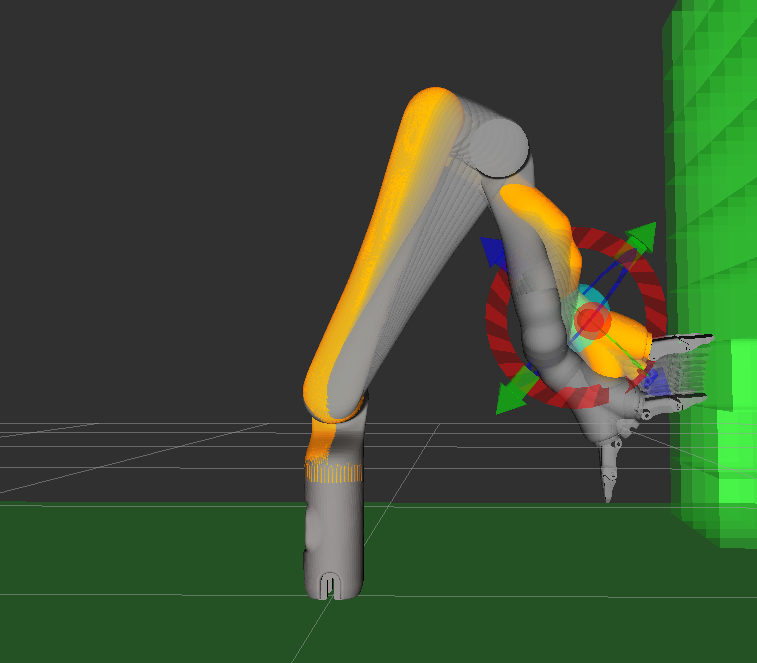
\includegraphics[width=\textwidth]{good_plan.png}
    \caption{}
    \label{fig:wrong_joint}
  \end{subfigure}

  \caption[Non-optimal motion plan]{When planning a small movement (10cm up) with KDL, motion plan (a) was produced; \REV{change of 1st joint} The solid gray arm is the start state, the orange arm the goal state, with the intermediate planned states in semi-transpareng gray}
  \label{fig:wrong_planning}
\end{figure}

This is caused by the KDL implementation. KDL finds the IK solution by iteratively descending the pose error by preforming its local linear approximation\cite{tracik}  and taking a step that minimizes it, analogic to the Newton method. The descent is performed by the inverse Jacobian method, but Moore-Penrose pseudoinverse is used in KDL because \quot{it is more efficient to compute}{tracik}, while it is numerically more stable when computed via SVD decomposition.

The descent can get trapped in local minima when some of the joints limits are reached. This is solved by restarting the search from a random seed position. Then, the found position can be one very distant from the original position in joint space.

This issue is tackled by a new IK solver released recently, TRAC-IK \cite{tracik}. The solver implements another approach to solving the IK problem by formulating it as a Sequential Quadratic Programming problem, minimizing cartesian error \(|e|^2\) with joint limits as constraints. The solver also allows the user to specify other constraints, like a wish to minimize joint-space distance between the seed (current arm joint values) and the result.

This setting allows us to eliminate the large joint space changes for minor movements, which was an issue with the JACO arm before.

A similar issue, which we failed to eliminate in the end, was caused by joint limit settings in the arm. While all the joint actuators allow continuous rotation (limited in software to \(\pm 27.7\) turns \cite{jaco_spec}) and only the second and third are limited by the arm design, when the arm is configured in MoveIt, a limit of \(\pm 1\) turn is imposed on the unlimited joints. The setup guide for TRADR project mentions limiting the joints is crucial to allow efficient planning. While this is true, it also causes artifacts like the path planned in Figure~\ref{fig:wrong_plan_joint}, where as in the previous case a tiny change in configuration needs seemingly unreasonably complex trajectory which is completely justified from the machine point of view, but looks nonsense to an observer.

\begin{figure}[htp]
  \centering
  \begin{subfigure}[t]{0.49\textwidth}
    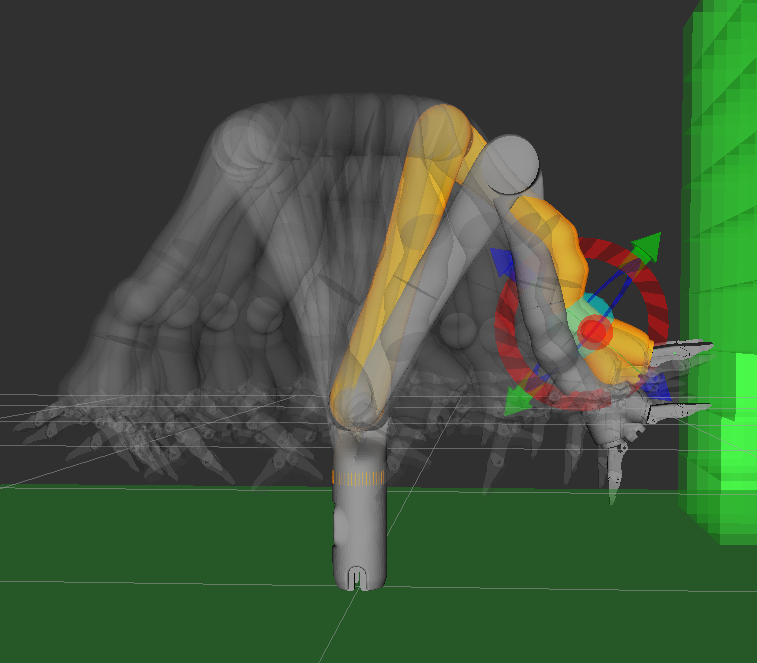
\includegraphics[width=\textwidth]{wrong_plan.png}
    \caption{}
    \label{fig:wrong_plan_joint}
  \end{subfigure}
  \begin{subfigure}[t]{0.49\textwidth}
    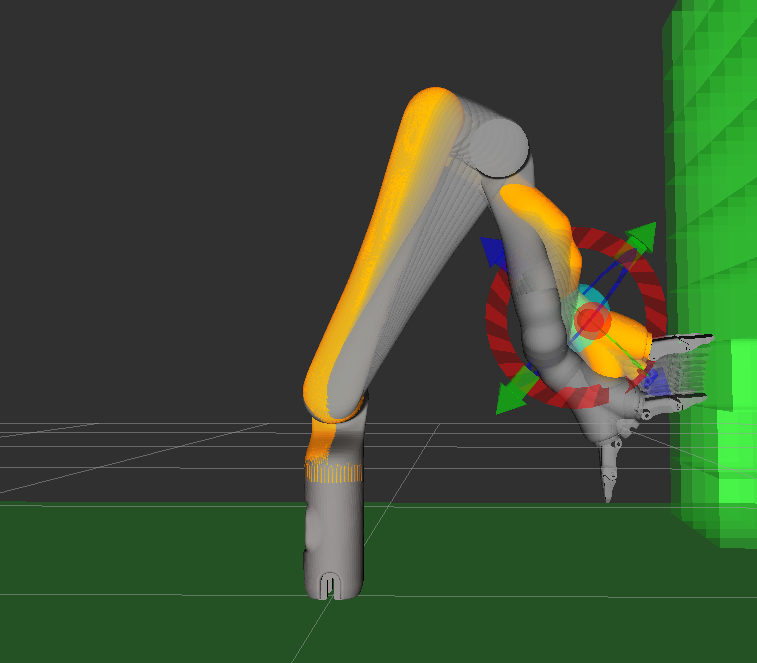
\includegraphics[width=\textwidth]{good_plan.png}
    \caption{}
    \label{fig:good_plan_joint}
  \end{subfigure}

  \caption[Non-optimal motion plan]{Motion plan affected by limited joints. In (a), the joint limit would be crossed if the arm took the straight path (b), and the IK solver and planner had no other chance than to perform full rotation in the first joint to stay within the limits. Plan (b) was generated after executing the first plan, which moved the arm away from the joint limit. The solid gray arm is the start state, the orange arm the goal state, with the intermediate planned states in semi-transparent gray}
  \label{fig:wrong_joints}
\end{figure}

\subsection{Motion planning}
\label{subsec:motion_planning}

Planning the motion of the manipulator in an environment with obstacles is a very complex task, suffering heavily from the curse of dimensionality. We are planning in 6-dimensional joint space from a given start pose to the target pose. Search-based planning algorithms fail because of the high dimension of the planning space, augmented by the need of fine space discretisation to keep the path smooth in the continuous real world.

Specialized planners based on sampling (Rapidly-exploring Random trees -- \emph{RRT} \cite{rrt}  or Kinodynamic Interior-Exterior Cell Exploration -- \emph{KPIECE}) are used to make planning the movement faster. The planners set constraints for the movement, like joint angle and velicity limits, collision checks etc. MoveIt has a plug-in interface to motion planning libraries, the default being OMPL \cite{ompl}, which implements a wide variety of algorithms, including the two mentioned here. Based on experiments with the arm and recommendations from \cite{vojta} and \cite{ompl}, we used the KPIECE family of planners, namely LBKPIECE, Lazy Bi-directional KPIECE.

% RRT build a tree that covers the configuration space. It starts as a single node, the start state. In each step of the expansion, a new configuration \m c is randomly sampled from the configuration space. Then, the node \m n nearest to \m c already in the tree is found, and the tree is expanded from \m n to a new node \m m in direction to \m c, while the movement from \m n to \m m must be entirely collision-free and within the constraints limiting e.g. the velocity. The expansion towards unexplored space drives very rapid exploration of the whole configuration space.

% KPIECE projects the configuration space into a grid, and then 

When a motion plan, a series of configurations from the start to the end, is computed, it is usually unnecessarily complicated, performing redundant movements. To smooth the trajectory out, the plan is simplified by a process in which states that are unnecessary, which means the path from their parent state to their child state satisfies the constraints as well, are removed. It is not unusual for a raw plan of movement of tens of centimeters to contain about two hundred states, which are later all removed, because the straight trajectory from the first to the second state is satisfactory.

\subsection{Moving the arm without planning}
\label{subsec:no_plan}

The problem with motion planning is that it is a complex task in itself, and, even though it is readily available as a part of MoveIt, it is slow and sometimes yields bad plans, even after employing the optimizing IK solver TRAC-IK\footnote{based on simple experiments not mentioned in this thesis, which consisted of simply moving the arm around with the motion planner}. In case of small movements, where a trivial linear path is often a good enough, if not optimal, solution, computing the whole huge motion plan is plain waste of resources and time.

The previous work \cite{vojta} used motion planning to carry out a simple downward motion, moving in 1\,cm steps. The same unnecessarily long paths have been reported.

It is not necessary to move the arm by following a motion plan. As we mentioned above, the Jacobian maps joint velocities \(\dot{\vec{q}}\) to Cartesian twist \(\vec{v}\)
\[
\mat J(\vec q) \dot{\vec{q}} = \vec v.
\]
Conversely, the Jacobian inverse (if it exists) maps Cartesian twist to joint speeds:
\[
\mat J^{-1}(\vec q) \vec v = \dot{\vec{q}}
\]

The inverse does not need to exist, or can be highly unstable as the Jacobian can be badly numerically conditioned. The near singularity of the Jacobian means that any of the null space of joint speeds would cause end effector movement in the desired direction. Or that the end of the end effector cannot be moved in the desired direction without requiring infinite speeds of the joints. In the second case, we need to leave the singularity in another direction.

In the first case, the problem is underconstrainted and can be solved for least square norm solution, which means the slowest joint motion. With advantage we use the Moore-Penrose pseudoinverse expressed in SVD decomposition of \(\mat J = \mat U \mat S \mat V^T \):
\[
\mat J^\dagger(\vec q) = \mat V \mat S^{-1} \mat U^T
\]
This approach gives us opportunity to check the conditioning of the operation, inspecting the singular values and zeroing out those that are below some threshold and could cause the solution to fail when inverted in constructing the pseudoinverse. The pseudoinverse then gives us the joint velocities directly:
\[
 \dot{\vec{q}} = \mat J^\dagger(\vec q) \dot{\vec{p}}
\]

We can then drive the robot along a trajectory with known speeds without expensive motion planning. A very simple example can be simple linear trajectories, where the cartesian velocity part of the twist is constant, and the angular part is zero.

%%%
\section{Tactile sensing}

Previous work in the field of tactile exploration at FEE \cite{vojta} used effort readings from the arm joints to detect tool contact when exploring terrain. To prevent arm damage, the movement had to be very slow, making it painstaking to explore event very little of the environment.

To improve exploration efficiency, we used a 3D force sensor to detect whether our tool is in contact with the environment. This allows us to move the arm much faster with confidence that we will be able to stop the arm with latency low enough to guarantee the arm nor the force sensor would be harmed.

\subsection{Optoforce sensor}
\label{subsec:opto}

The force sensor used is an Optoforce OMD-20-SE-40N sensor. Optoforce sensors represent a novel approach to 3D force sensor construction, as their working principle enables them to be made very rugged, resilient.

\begin{figure}[ht]
  \begin{subfigure}[t]{0.4\textwidth}
    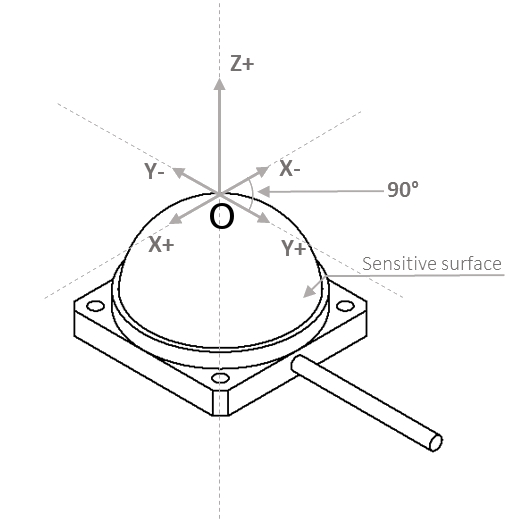
\includegraphics[width=\textwidth]{OMD-sketch-with-axises}
    \caption{}
    \label{fig:omd_geom}
  \end{subfigure}
  \begin{subfigure}[t]{0.4\textwidth}
    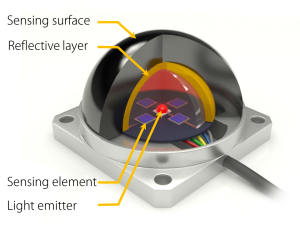
\includegraphics[width=\textwidth]{OMD-xsec}
    \caption{}
    \label{fig:omd_xsec}
  \end{subfigure}

  \caption[Optoforce sensor]{The optoforce sensor reference frame (a) and cross-section (b). Taken from \cite{opto_whitep}}
  \label{fig:decomps}
\end{figure}

The Optoforce sensor, seen in cross-section in Figure~\ref{fig:omd_xsec}, consists of an aliminium base plate, made in different designs, and a hollow silicone hemispherical dome. The interior of the dome is coated with a reflective layer. A light emitter, IR LED, is positioned on the base plate in the center of the dome. Four light-sensitive diodes are placed around it.

When the sensor is operational, the LED emits light which bounces around the dome and provides known, constant illumination on the photodiodes. When force is applied to the dome, it deforms, and the deformation causes the illumination of the diodes to shift. From this shift, it is possible to determine the direction in which the force has been applied. According to the manufacturer, deformations in range of hundreds of nanometers can be measured \cite{opto_whitep}. After some time in operation, the sensor occasionaly gets confused and reports rather large false forces (up to 10N on z axis). A strong compression of the dome resets the sensor to correct readings.

The sensor has its own DAQ (\emph{Data AcQuisition}) module, which communicates with a computer via a serial link emulated over USB. The manufacturer provides a C++ library that exposes the sensor functionality in an API. It however depends on the problematic Qt framework. Shadow Robot Company \cite{opto_driver}  implemented a ROS node that connects to the sensor serial interface, configures sensor parameters like measurement and filter frequency, reads the data output by the sensor and publishes them on a ROS topic to be processed by other components. The readings published are in Newtons, as the driver is provided with a \uvz{sensitivity report}, a calibration result provided by the manufacturer that relates the internal units used by the sensor to actual physical forces. The driver software was released under GPLv2. We simplified the driver and slightly adjusted it to work better in our setup.


\section{Contributions to the hardware and framework}
\label{sec:hw_contrib}

\subsection{Arm simulator}
\label{subsec:arm_sim}

To simplify development, we implemented a mock arm driver mimicking the Kinova ROS driver. The mock driver is meant to be used with MoveIt! as a drop-in replacement of the original driver, and hence it only implements FollowJointTrajectory action. It receives a joint speed trajectory, and replays it, publishing mock arm configuration to the respective topic where the rest of the system expects robot joint readings. Then, the rest of the system cannot distinguish the mock arm and the real robot.

The mock driver can be configured to execute the joint trajectories faster, to save time the user spends watching the simulated arm move. The mock driver does not simulate arm dynamics in any way, it only tries to follow the trajectory in the same way as the real driver does. In the end, instead of being driven by a regulator to the real target angles, we set the joint angles directly.

The simulator also mimicks the driver's ability to drive the arm by specifying joint speeds. It reads a joint velocity input at 100\,Hz, behaving exactly as the real driver as described in \ref{subsec:api_cart_vel}.

This simulator allows us to test the system without the need of using, driving and taking care of a expensive physical arm.


\subsection{Sensing tool and measurement processing}
\label{subsec:sense_tool}

The Optoforce sensor is relatively small. Mounting it on the JACO arm and using it to sense direct contact with an obstacle would mean the arm would get uncomfortably close to it. We devised a way to extend the sensor so that force readings are taken not at the sensor dome, but at a stick. This increases the arm range and makes it possible to keep the arm safely away from unknown obstacles.

The sensor is mounted in a frame together with a stick. The stick ends at the sensor with a specially designed cap that transfers forces from the stick to the dome of the sensor itself. The other end of the stick is blunted not to be dangerous to its surroundings.

\begin{figure}[htp]
  \centering

  \begin{subfigure}[t]{0.44\textwidth}
   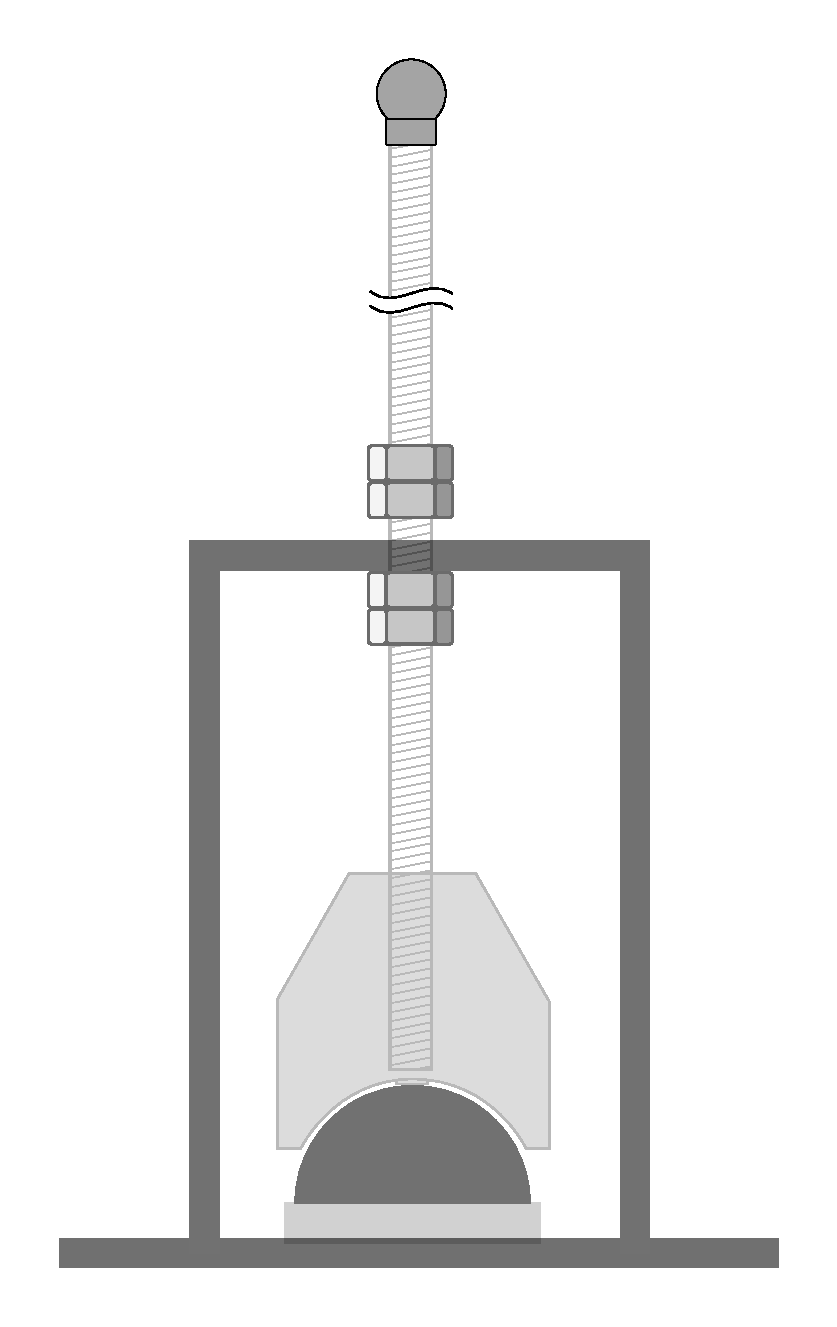
\includegraphics[width=\textwidth]{otpo_frame.pdf}
   \caption{\label{fig:opto_frame}}
  \end{subfigure}
  %
  \begin{subfigure}[t]{0.44\textwidth}
   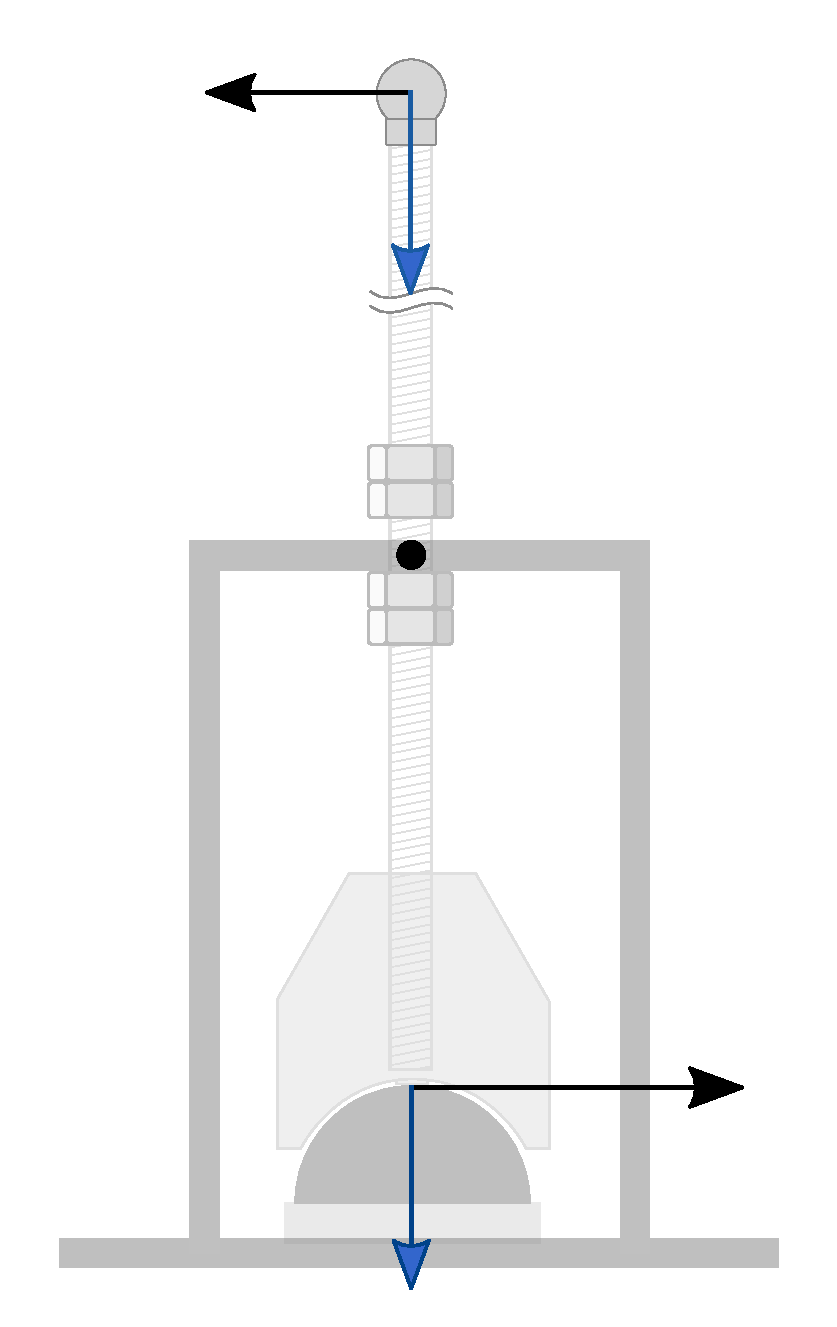
\includegraphics[width=\textwidth]{otpo_frame_forces.pdf}
   \caption{\label{fig:frame_forces}}
  \end{subfigure}

 \caption[Sensing tool]{The sensing tool assembly in cross-section (a) and forces in the instrument (b)}
 \label{fig:opto_frame_fig}
\end{figure}


\begin{figure}[htp]
  \centering
  \hspace{2cm}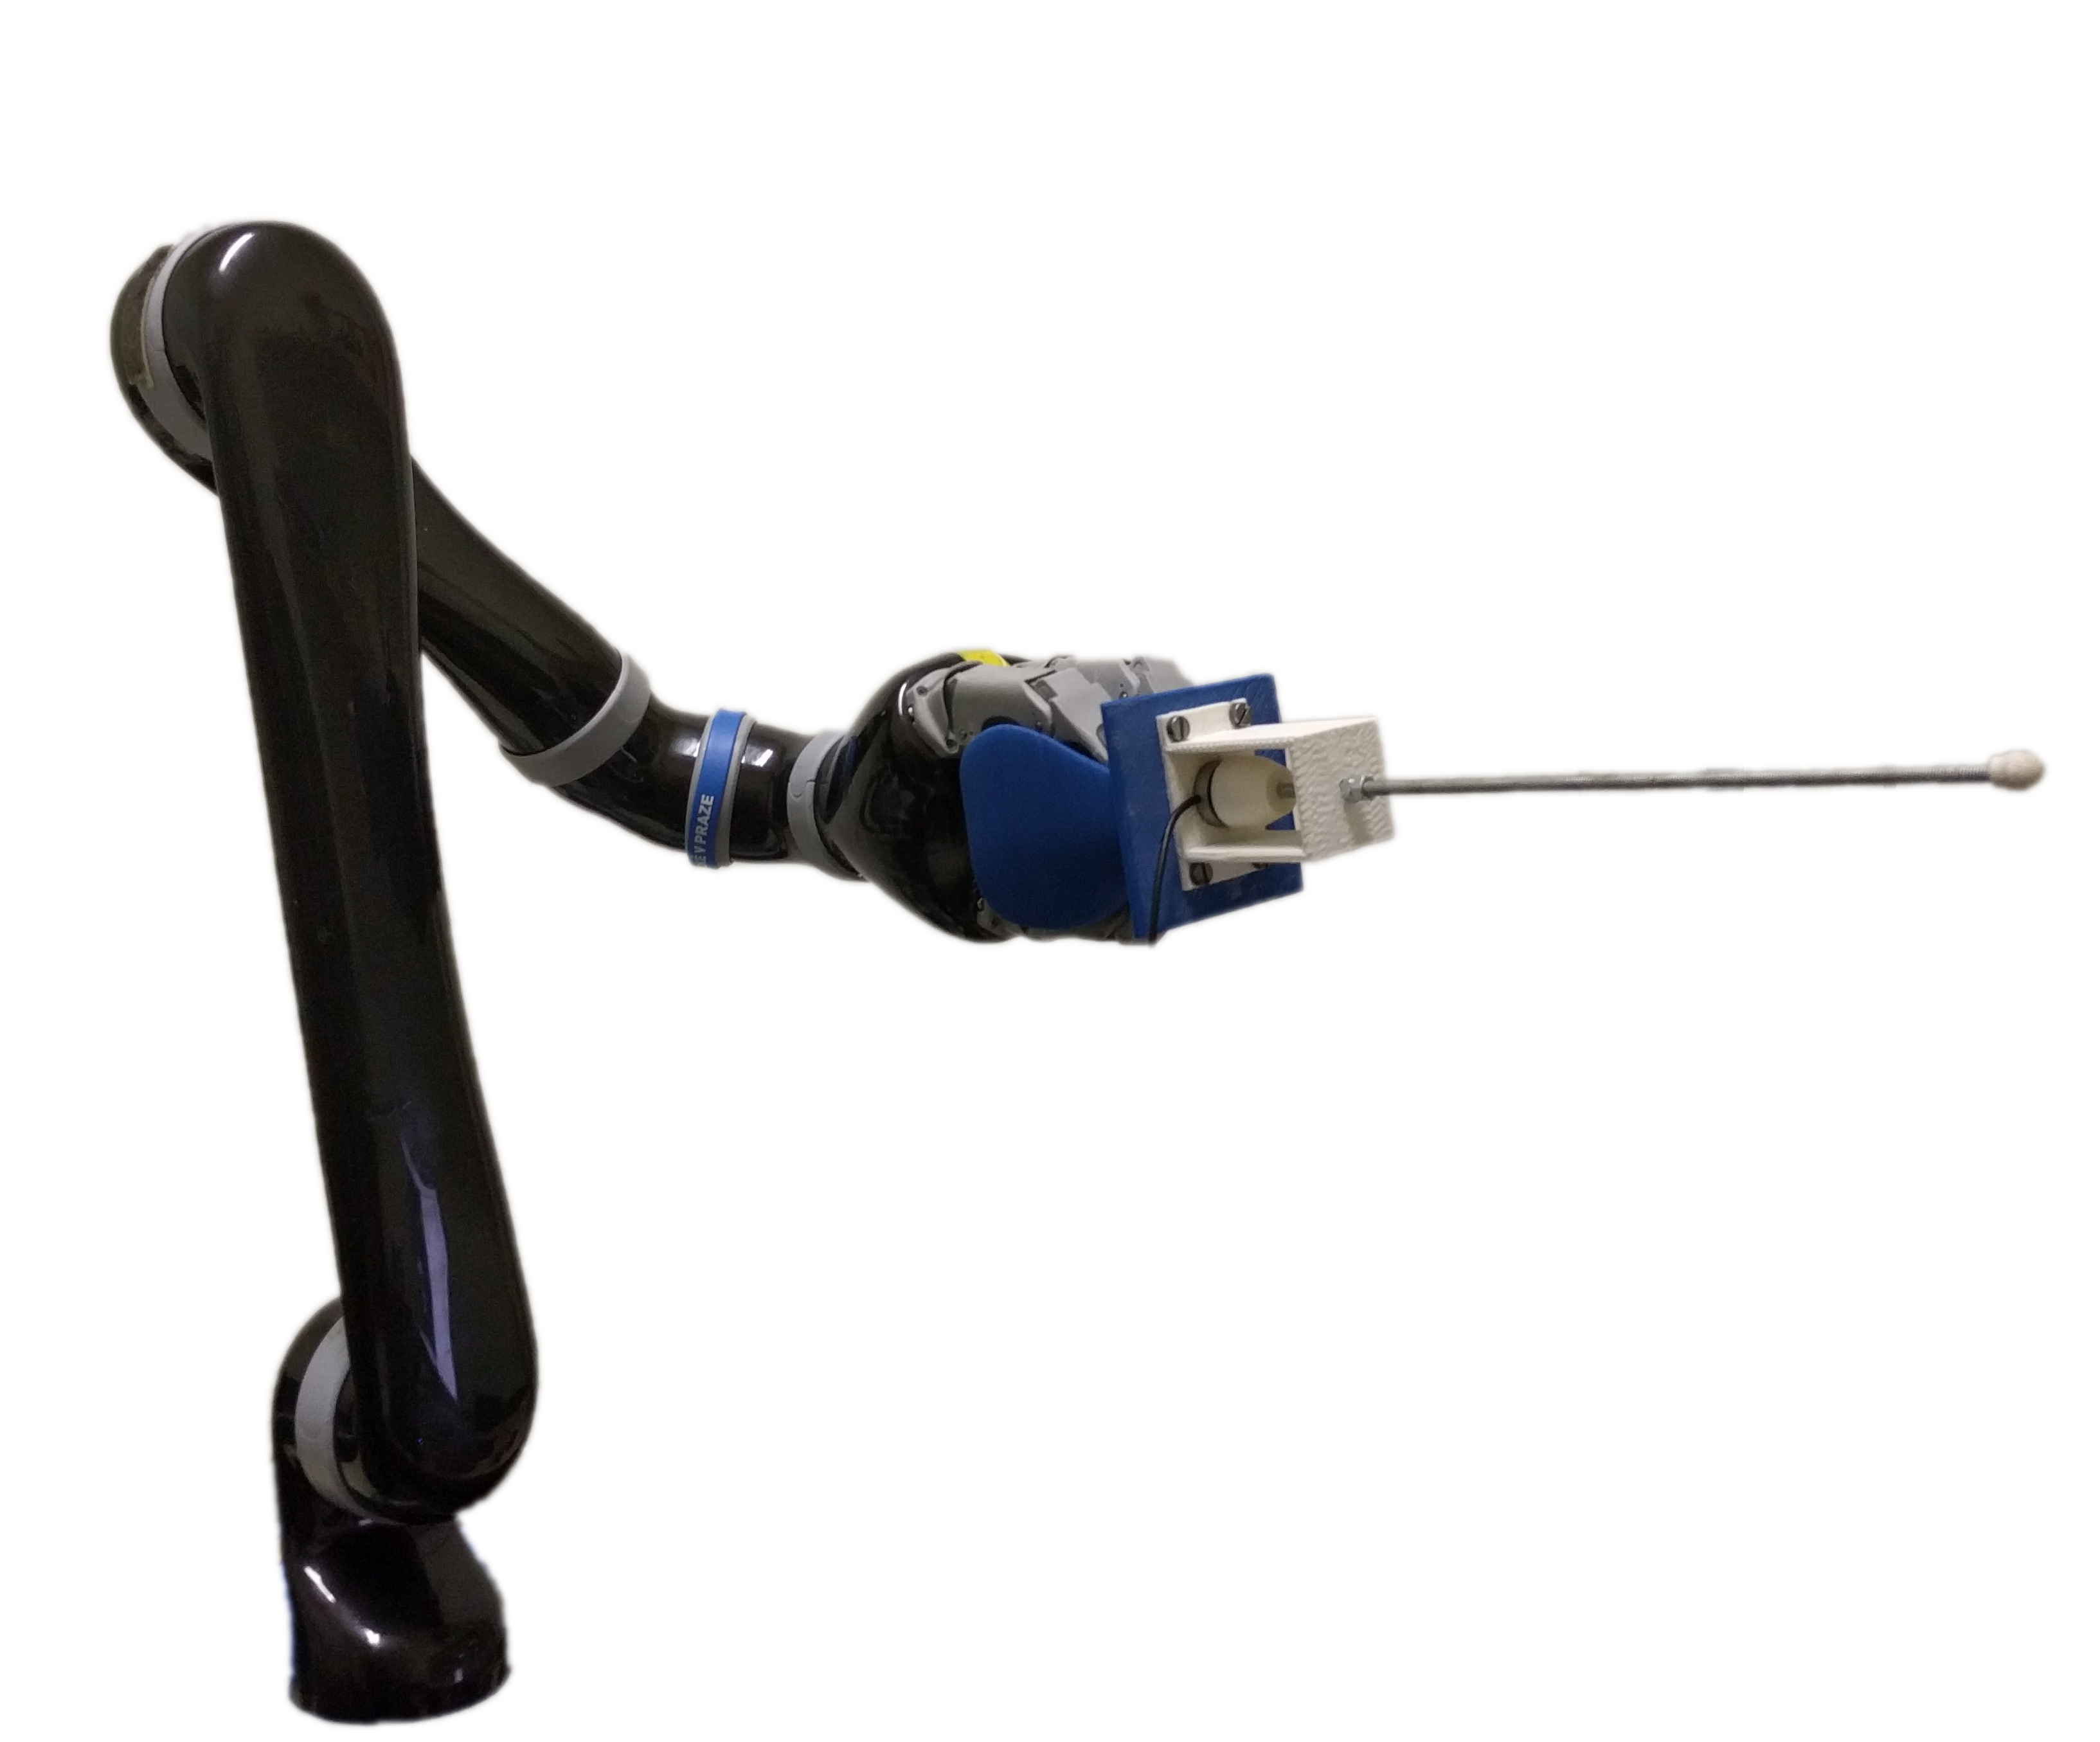
\includegraphics[width=8cm]{jaco_base.png}
  \caption[Sensing tool]{The sensing tool held in the JACO arm's gripper}
  \label{fig:tool_photo} 
\end{figure}

The stick acts as a lever with the pivot point being the assembly frame. When a lateral force is applied to the stick, the sensor records force in opposite direction. Axial force is applied directly to the sensor. The principle is illustrated in Figure~\ref{fig:frame_forces}.

The sensor dome is in contact with a cap attached to the stick. The cap is pressed against the dome with a preloaded force, to ensure accurate measurement of even very small forces applied to the stick. The deformation of the dome is limited by a pair of nuts that limit the travel of the stick.

The whole assembly is mounted to a lump of plastic ergonomically designed for the JACO 3-finger gripper, so that the sensor can be attached to the hand without any hassle and operatively, and could, in theory, be mounted somewhere on the robot and taken by the arm automatically only when necessary.

\begin{figure}[ht]
  \centering
  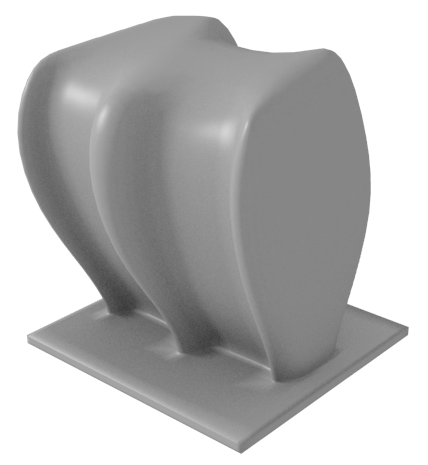
\includegraphics[width=7cm]{lump.png}
  \caption[Tool grip handle]{The ergonomic grip handle we designed to facilitate mounting hardware onto the arm. The square base can be used to mount any object to the handle in the future. The 3-finger gripper on the arm can hold it firmly enough to withstand considerable force}
  \label{fig:label}
\end{figure}

The sensor is connected to the DAQ and then the computer through external cables. This limits the arm, as for example a full joint rotation would wind the cable around a link. For this reason, we left the cable free from the arm and used it only when the experiment needed it. In the arm, a builtin pass-through cable is available, which would eliminate the external cable and allow us to fully use the arm. We however do not have the means to use the cable to transfer sensor data, although we hope it will be possible in the future.

The measurements from the sensor are processed by other components of the system. By observing the data obtained by hte sensor during random movement of the arm (no contact with the stick), the gravitational force of the stick itself, combined with vibrations, can cause lateral forces of up to 1\,N. We recommend to detect contact by thresholding the contact force by 2\,N for the lateral forces and 4\,N for axial forces.

\end{document}

%%% Local Variables:
%%% mode: latex
%%% TeX-master: "buriama8_dp"
%%% End:
